\section{Introduction}
\label{sec:introduction}

\IEEEPARstart{R}{obotic} tool use on deformable and flowable media---scooping granular piles, pushing viscous pastes, transferring cohesive snow-like aggregates---requires adapting manipulation to hidden physical properties that are not visible in a single snapshot. Two materials that look nearly identical to a camera can differ by an order of magnitude in stiffness, cohesion, or flow resistance, and the manipulation strategy that succeeds on one of them can fail catastrophically on the other~\cite{huang2022plasticinelab,lin2022diffskill,shi2023robocook}. A robot that relies only on instantaneous observations therefore faces an inherently under-constrained control problem: the same observed state can correspond to many distinct dynamics.

A common response is to train reactive policies with domain randomization~\cite{tobin2017domain,peng2018sim2real} or to use a history-conditioned recurrent policy~\cite{hausman2018learning,xie2018learning}. These approaches trade breadth for depth---they spread the policy thin across many material instances without ever explicitly inferring what material the robot is currently manipulating. An alternative is discrete material classification followed by per-class policy routing~\cite{calandra2018more}, which requires a closed set of material labels and brittle perception. Neither strategy offers an explicit mechanism for the robot to \emph{ask the physics a question} before committing to a manipulation plan.

We take a different position: \emph{manipulation under hidden material properties should include an explicit, short information-gathering interaction whose response is encoded into a latent vector that conditions the downstream policy}. Humans probe unfamiliar substances before picking them up and use the response to pick a grasp and a motion profile. We operationalize this intuition in \PTA{} (\cref{fig:hero}). \PTA{} is deliberately minimal: the probe is a fixed open-loop trajectory, the encoder is a small MLP, and the residual policy is standard PPO. The active component of \PTA{} is the budgeted allocation of an initial interaction segment and the learned downstream use of its response; the probing action itself is not optimized as an information-gathering policy. The contribution of this paper is therefore empirical and diagnostic---a study of when this minimal probe-conditioning helps versus hurts deformable-material manipulation---not a new inference architecture.

\begin{figure*}[t]
    \centering
    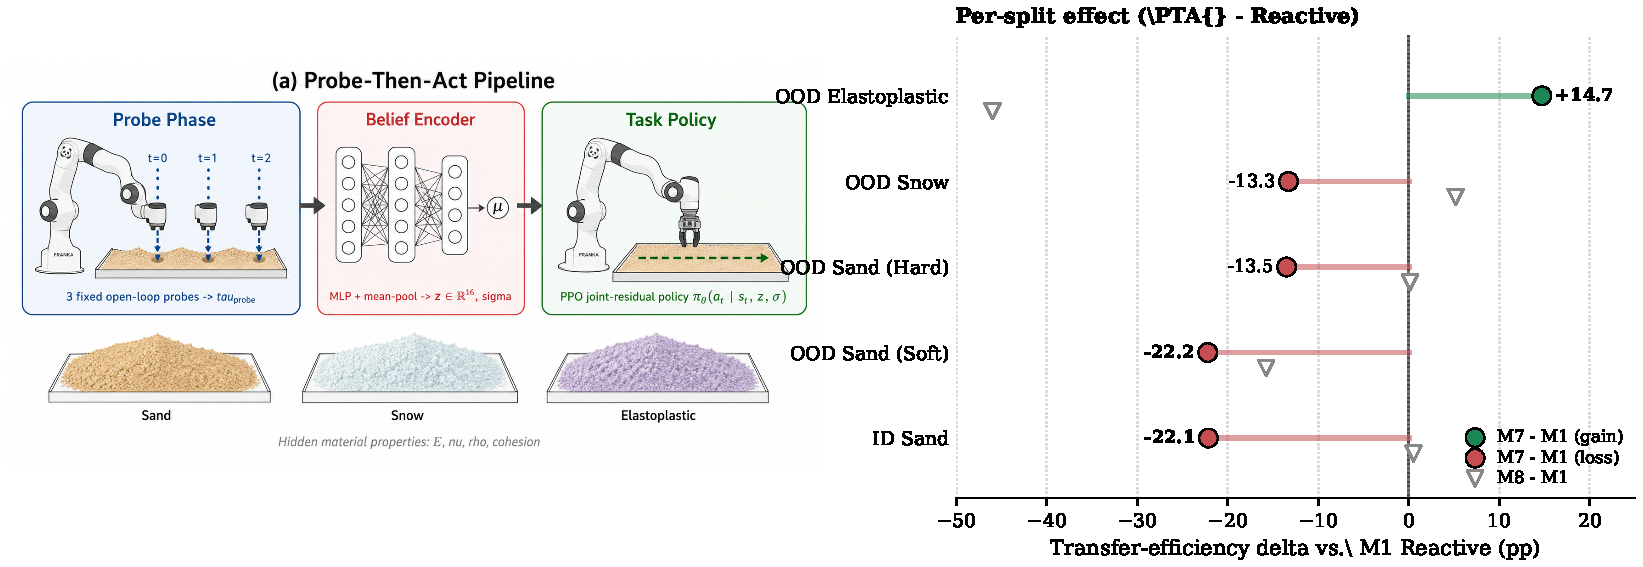
\includegraphics[width=0.98\textwidth]{figures/fig1_hero.pdf}
    \caption{\textbf{\PTA{} framework and per-split effect.} Left: schematic illustration of the two-stage architecture --- (i) the robot executes a short fixed open-loop probing phase, (ii) an encoder maps the probe trace to a latent task-conditioning vector $z$ with a learned scale parameter $\sigma$ (not a calibrated posterior), (iii) the task policy is conditioned on $(s_t, z, \sigma)$ to produce adaptive joint-space residual actions. Material piles below the schematic illustrate the three Genesis MPM families used in the benchmark; the schematic is for explanation and is not a Genesis render (Genesis renders appear in \cref{fig:scene_schematic}). Right: per-split transfer-efficiency delta of \PTA{} (M7) versus the matched reactive baseline (M1), in percentage points; hollow downward markers show the M8 privileged-parameter delta. \PTA{} wins by $+14.7$\,pp on OOD elastoplastic and underperforms on the four other splits ($-13$ to $-22$\,pp), with M8 collapsing to $-46$\,pp on elastoplastic. Means over 3 training seeds, 10 evaluation episodes per seed; this overview shows mean deltas only and the comparison is descriptive, not significance-tested. Matched-seed dispersion is shown in \cref{fig:seeds}; absolute values for all three methods are in \cref{fig:main}.}
    \label{fig:hero}
\end{figure*}

\begin{enumerate}
    \item \textbf{Probe phase.} The robot executes a short, fixed open-loop sequence of exploratory contacts with the material while the task residual is held at zero. The resulting proprioceptive and aggregate-particle trace implicitly encodes the material's response to applied forces.
    \item \textbf{Encoder.} An MLP with mean-pooling maps the probe trace to a latent task-conditioning vector $z \in \R^{16}$ and a learned scale $\sigma$. We refer to $(z, \sigma)$ as a ``belief'' for brevity, but the pair is not a calibrated posterior: there is no KL regularizer, prior, or auxiliary classification loss; $z$ is whatever representation of the probe response is task-useful under the end-to-end PPO objective.
    \item \textbf{Task policy.} A joint-residual PPO policy is conditioned on $(s_t, z, \sigma)$ and emits joint-space residuals on top of a scripted edge-push base trajectory. The base trajectory sidesteps differentiable-IK coupling artifacts we observed in the simulator~\cite{genesis2024}.
\end{enumerate}

\paragraph{The recoverable-deformation hypothesis.}
Probing is not free: every probe step displaces particles, breaks contacts, and consumes task time. We offer a physics-grounded interpretation of when this cost is likely to pay off, treated throughout as an \emph{interpretive hypothesis} rather than a demonstrated principle:
\begin{quote}
\emph{Active probing should be expected to help downstream manipulation only when the material's response to a probe is \textbf{recoverable}---the probed configuration relaxes back, on the task timescale, to a state the policy can still exploit---and to be net-negative when probe-induced perturbations are \textbf{irreversible}.}
\end{quote}
Elastoplastic media in our benchmark exhibit recoverable elastic rebound; granular sand (especially under low cohesion) exhibits irreversible rearrangement. The hypothesis therefore anticipates, and our experiments are consistent with, gains on elastoplastic and losses on the granular splits, with cohesive snow in between.

\paragraph{Empirical evaluation.}
We evaluate \PTA{} on a reproducible cross-material edge-push benchmark in Genesis~\cite{genesis2024} spanning sand (granular, 32\% scripted transfer), snow (cohesive, 87\%), and elastoplastic medium with recoverable elastic rebound (70\%), plus two parameter-shifted sand variants. The 55-percentage-point scripted-transfer spread is discriminative by design. All methods are trained on the hardest split (sand) only and evaluated zero-shot on the other four, so the encoder is asked to \emph{extrapolate} rather than to interpolate over a labeled material mix.

On the elastoplastic split, \PTA{} achieves $60.7$\% transfer versus $46.0$\% for a matched reactive PPO baseline (M1)---14.7pp absolute, 32\% relative---accompanied by a 14.7pp reduction in spillage (39.3\% vs.\ 54.0\%; \cref{tab:main_results}, \cref{fig:main}). Matched ablations indicate both probe and encoder are necessary for this elastoplastic improvement: removing the probe drops transfer by 27.6pp and removing the encoder output drops it by 14.4pp, with both ablations falling below the reactive baseline (\cref{tab:ablation}). On the four other splits \PTA{} underperforms by 13--22pp, including a 22pp loss on in-distribution sand. We do not claim broad cross-material robustness; we report a 1-of-5 conditional win whose direction is anticipated by the recoverable-deformation hypothesis on every split. A complementary observation: a privileged-parameter baseline (M8) that receives ground-truth material parameters collapses to 0\% transfer on elastoplastic across all three seeds while remaining strong elsewhere. We read this narrowly---in our sand-only-trained, residual-control setup, a passive parameter vector did not unlock a learned response curve for elastoplastic rebound while a probe-induced response did---and not as a universal claim about privileged information.

\paragraph{Contributions.} We make three contributions, framed as empirical and diagnostic:
\begin{enumerate}
    \item A \textbf{conditional empirical finding}: on a discriminative cross-material benchmark, a minimal probe-then-act policy beats a matched reactive PPO baseline on one OOD recoverable-rebound split (+14.7pp transfer, $-$14.7pp spill on elastoplastic) while underperforming by 13--22pp on the four other splits, with matched ablations placing probe and encoder \emph{below} the reactive baseline when either is removed.
    \item A \textbf{recoverable-deformation hypothesis}, offered as a physically motivated interpretation rather than a demonstrated principle---a candidate boundary condition for active probing, to be tested in future work on additional viscoelastic and granular media.
    \item A \textbf{reproducible cross-material benchmark} in Genesis with five splits (55pp of scripted-transfer spread), standardized 3-seed protocol, per-seed metrics, and ablation infrastructure; code and seeds will be released upon acceptance.
\end{enumerate}

\paragraph{Scope of claims.}
\PTA{} as evaluated here uses a fixed open-loop probe, observations that include simulator-derived aggregate-particle statistics, and an end-to-end task-conditioning latent without calibration or material-label supervision; all training is on sand. We therefore treat the results as a \emph{diagnostic} study of when a minimal probe-conditioned policy helps, not as a complete sensing or broadly robust manipulation system.

The rest of the paper is organized as follows. \cref{sec:related} positions our work against active perception, deformable manipulation, system identification, and multi-physics benchmarks; \cref{sec:method} formalizes \PTA{}; \cref{sec:experiments} describes the benchmark and evaluation; \cref{sec:results} reports the main results and ablations; \cref{sec:discussion,sec:conclusion} discuss scope, limitations, and conclude.
